\chapter{Linear Models: Analysis of variance}
\label{ch:ANOVA}

Aims of this chapter \footnote{Here you work with the script file {\tt anova.R}}:
\begin{compactitem}
	\item Plotting boxplots and barplots using factors
	\item Fitting factors in linear models using analysis of variance
	\item Diagnostic plots for explanatory factors
	\item Exploring differences between levels of a factor
\end{compactitem}

\section{What is ANOVA?}

\begin{figure}
	\centering
	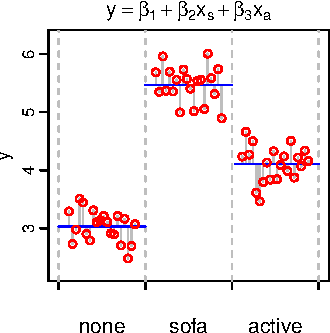
\includegraphics[width=.4\textwidth]{ANOVA_is_LM.pdf} 

	\caption{A dataset where an ANOVA would be appropriate. performing an 
	ANOVA test on this dataset is the same as fitting the linear model  
	$y  = \beta_1  + \beta_2 x_s + \beta_3 x_a$, where $x_s$ and $x_a$ 
	are two levels. There are three ``treatments'' here with the first 
	treatment, the control, captured by the baseline value $\beta_1$ 
	(the sample with the lowest value, on the far left)}

	\label{fig:anova1} 

\end{figure}

A {\it One-way analysis of variance} (one-way ANOVA) is a technique 
used to compare means of two or more samples representing numerical, 
continuous data. 

ANOVA tests the null hypothesis that samples from two or more groups 
are drawn from populations with the {\it same mean value}. To do this, 
ANOVA uses the {\it F}-statistic --- the ratio of the variance 
calculated across the samples (groups) (the null hypothesis) to the 
variance within the samples (groups). If the null hypothesis that the 
group means are drawn from populations with the same mean is indeed 
true, the between-group variance (numerator in the F-ratio) should be 
lower than the within-group variance (denominator). A higher ratio (and 
{\it F} value) therefore implies that the samples were drawn from 
populations with different mean values.

This is same as asking whether a linear model with a predictor (or 
explanatory variable) with at least two categorical levels (or 
factors), better accounts for the variance (Explained Sum of Squares, 
ESS) than a null model of the form $y  = \beta_1$ (Figure 
\ref{fig:anova1}). Thus, ANOVA is just a type of linear model. 

By the end of this chapter, it will make more sense to you how/why 
linear regression models that we covered in Chapter \ref{ch:regress}, 
of the form $y = \beta_1  + \beta_2 x$ (where $x$ is a continuous 
predictor variable),  require ANOVA to determine if the the model 
better fits than a null model of the form $y  = \beta_1$.

Typically, one-way ANOVA is used to test for differences among at least 
three groups, since the two-group (or levels or factors) case can be 
covered by a $t$-test (see Chapter~\ref{ch:t_F_tests}). When there 
are only two means to compare, the $t$-test and the F-test are 
equivalent; the relation between ANOVA and t is given by $F = t^2$. 

An extension of one-way ANOVA is two-way analysis of variance that 
examines the influence of two different categorical independent 
variables on one dependent variable --- we will look at multiple 
predictor variables in Chapter \ref{ch:MulExpl} onwards.

\section{Calculating the ANOVA test statistic}

ANOVA ``partitions'' variability in your data as follows: 

\begin{description}

	\item[Total sum of squares (TSS)] This is sum of the squared 
	difference between the observed dependent variable ($y$) and the mean 
	of the response variable $y$ (denoted by $\bar{y}$), i.e., 
	$$\text{TSS} = \sum_{i=1}^{n}(y_i - \bar{y})^2$$ TSS tells us how 
	much variation there is in the dependent variable without having any 
	other information (your null model). You might notice that TSS is the 
	numerator of the sample variance you learned about in Chapter 
	\ref{ch:ExpDesign}.
  
	\item [Explained sum of squares (ESS)] Sum of the squared differences 
	between the predicted $y$'s (denoted $\hat{y}$'s) and $\bar{y}$, or, 
	$$\text{ESS} = \sum_{i=1}^{n} (\hat{y}_i - \bar{y})^2$$ ESS tells us 
	how much of the variation in the dependent variable our alternative 
	(linear) model was able to explain. That is, it's the reduction in 
	uncertainty that occurs when the linear model is used to predict the 
	responses.
	
	\item [Residual sum of squares (RSS)] Sum of the squared differences 
	between the observed $y$'s (denoted by $y_i$) and the predicted 
	$\hat{y}$, or, $$\text{RSS} = \sum_{i=1}^{n} (\hat{y}_i - y_i)^2$$ 
	RSS tells us how much of the variation in the dependent variable our 
	model could not explain. That is, it's the uncertainty that remains 
	even after the linear model is used. The linear model is considered 
	to be statistically significant if it can account for a large amount 
	of variability in the response.

\end{description} 

And of course, TSS = ESS + RSS; the OLS method ``decomposes'' the total variation in the dependent variable into an explained component (ESS; explained by the predictor) and an unexplained or residual component (the RSS). 

These sums of squares can then be used to calculate the statistical 
significance of the linear model (Regression, ANOVA, etc) through the 
F-Value (or F-Ratio), as follows: 

\begin{center}
\def\arraystretch{1.5}
\begin{tabular}{|>{\centering}m{2cm}|>{\centering}m{2.1cm}|>{\centering}m{2cm}|>{\centering}m{2cm}|p{1.5cm}|}
\hline
Type of Sum of Squares (SS)  & Calculation & Degrees of Freedom (DF) & 
Mean Sum of Squares (MSS) & F-Value \\ \hline

TSS & $\sum_{i=1}^{n}(y_i - \bar{y})^2$   & $n-1$ &$\frac{TSS}{n-1}$& 
\multirow{3}{*}{ 
$\frac{\left(\frac{ESS}{n_c-1}\right)}{\left(\frac{RSS}{n-n_c}\right)}$} \\ \cline{1-4}

ESS & $\sum_{i=1}^{n} (\hat{y}_i - \bar{y})^2$ & $n_c-1$ & $\frac{ESS}{n_c-1}$ &  \\ \cline{1-4}

RSS & $\sum_{i=1}^{n} (\hat{y}_i - y_i)^2$ &  $n-n_c$ &  $\frac{RSS}{n-n_c}$ & \\ \hline
\end{tabular}
\end{center}

\subsection{Degrees of freedom}
Thus each sum of squares has a corresponding degrees of freedom (DF) 
associated with it that gives the Mean Sum of Squares (MSS)  --- the Sums of Squares divided by the corresponding degrees of freedom.

The TSS DF is one less than the number of observations $n-1$. This is because calculating TSS, needs $\bar y$ , which imposes loss of one degree of freedom. Note that MSS is thus nothing but the sample variance.

The ESS DF is one less than the number of coefficients ($n_c$) 
(estimated parameters) in the model: $n_c-1$. Note that in the case 
where the linear model is an ANOVA, it the number of coefficients 
equals the number of ``treatments'' (the categories or levels in the 
predictor). So for example, in Fig. \ref{fig:anova1}, there are three 
treatments (predictors) and therefore three coefficients ($\beta_1$, 
$\beta_2$, $\beta_3$), which means that the ESS degrees of freedom 
there is $n_c-1 = 2$. 

The RSS DF is the sample size $n$ minus the number of coefficients $n_c$, that is, $n - n_c$, because each estimated coefficient is an unknown parameter.

\subsection{The F-Value (or Ratio)}

Finally, The F-Value or F-Ratio, the test statistic used to decide 
whether the linear model fit is statistically significant, is the ratio 
of the Mean ESS to the Mean RSS. The null hypothesis is rejected if the 
F-ratio is large --- the model explains a significant amount of 
variance. The p-value is then calculated from the F-distribution as you 
learned before, in Chapter \ref{ch:t_F_tests} (see Fig. \ref{fig:fdist}).  

Also note that the Root Mean Square Error (RMSE), also known as the 
standard error of the estimate, is the square root of the Mean RSS. It 
is the standard deviation of the data about the Linear model, rather 
than about the sample mean.

\subsection{The $R^{2}$}

Finally, $R^{2}$, also called the Coefficient of Determination, is the 
proportion of total error (TSS) explained by the model (ESS), so the 
ratio ESS/TSS. That is it is the proportion of the variability in the 
response that is explained by  by the fitted model. Since TSS = ESS + 
RSS, $R^{2}$ can be rewritten as (TSS-RSS)/TSS = 1 - RSS/TSS. If a 
model has perfectly fits the data, $R^{2}=1$, and if it has no 
predictive capability $R^{2}=0$. In 
reality, $R^{2}$ will never be exactly 0 because even a null model will 
explain some variance just by chance due to sampling error. Note that 
$R$, the square root of $R^2$, is the multiple correlation coefficient: 
the correlation between the observed values ($y$), and the predicted 
values ($\hat{y}$).

As additional predictors (end therefore linear model coefficients) are 
added to a linear model, $R^2$ increases even when the new predictors 
add no real predictive capability. The adjusted-$R^2$ tries to addresses this 
problem of over-specification or over-fitting by including the degrees 
of freedom: Adjusted $R^2$ = 1 - (RSS/$n-n_c-2$)/(TSS/$n-1$) 
\footnote{That is, it is 1 minus the ratio of the square of the 
standard error of the estimate to the sample variance of the response}. 
Thus additional predictors with little explanatory capability will increase 
the ESS (and reduce the RSS), but they will also have lower RSS degrees of 
freedom (because of the additional number of fitted coefficients, 
$n_c$'s)\footnote{i.e., Standard error of the estimate won't 
decrease}. Thus if the additional predictors have poor predictive 
capability, these two reductions will cancel each other out. In other 
words, the Adjusted $R^2$ penalizes the addition of new predictors to 
the linear model, so you should always have a look at the Adjusted 
$R^2$ as a corrected measure of $R^2$.   

\section{A new dataset}

In this Chapter, we will use a new dataset of genome size and life 
history in mammals to try out a one-way ANOVA. The dataset is a 
composite of data taken from an online database of genome sizes and a 
published database of mammalian life history:

\begin{compactdesc}
	\item[Genome size] Average genome sizes for available mammal species 
	are taken from the online database  
	\href{www.genomesize.com}{www.genomesize.com}.
	\item[Life history] Trait data for these species are taken from: 
	\href{http://esapubs.org/archive/ecol/e090/184/metadata.htm}{
	Jones, K. E. {\it et al.} (2009) PanTHERIA: a species-level database 
	of life history, ecology, and geography of extant and recently 
	extinct mammals. Ecology 90, 2648--2648}.
\end{compactdesc}

\begin{compactitem}[$\quad\star$]
	\item Download the file {\tt MammalData.csv} from bitbucket and save 
	to your {\tt Data} directory.
	\item Create a new blank script called {\tt ANOVA\_Prac.R} and add 
	some introductory comments.
	\item Use {\tt read.csv} to load the data in the data frame 
	{\tt mammals} and then {\tt str} and {\tt summary} to examine 
	the data.
\end{compactitem}

There are nine variables. The first two are the latin binomial and 
taxonomic order of each species, followed by the species mean genome 
size (`C value', picograms), adult body mass (g), diet breadth, habitat 
breadth, litter size and then two factors showing whether the species 
are ground dwelling and their trophic level. For more information, see 
the link above.

You will see from the output of {\tt summary} that there is lots of 
missing data for the life history traits.

\section{Exploring the data with boxplots}

We are interested in finding out whether the mean C value for species 
varies predictably for different levels of life history traits (a 
typical one-way ANOVA question). For example: 

\begin{compactitem}
\item Do carnivores or herbivores have larger genome sizes?
\item Do ground dwelling mammals have larger or smaller genome sizes?
\end{compactitem}

Before we fit any models, we want to plot the data to see if the means 
within these groupings look different. We also want to check whether 
the variance looks similar for each group: {\it constant normal 
variance}! A simple way is to look at box and whisker plots, showing 
the median and range of the data:

\begin{compactitem}[$\quad\star$]
	\item Use {\tt plot(meanCvalue \textasciitilde{} TrophicLevel, 
	data= mammals)} to generate a boxplot of the differences in genome 
	sizes between trophic levels.
	\item Looking at the plots, it is clear that there is more spread in 
	the data above the median than below. Create a new variable {\tt 
	logCvalue} in the {\tt mammals} data frame containing logged C 
	values.
	\item Create a boxplot of log C values within trophic groups.
	\item Repeat the two plot commands to look at differences between 
	ground dwelling and other species.
\end{compactitem}

\section{Differences in means with barplots}

Box and whisker plots show the median and spread in the data very 
clearly, but we want to test whether the means are different. This is 
$t$ test territory --- how different are the means given the standard 
error --- so it is common to use barplots and standard error bars to 
show these differences.

We're going to use some R code to construct a barplot by hand. We need 
to calculate the means and standard errors within trophic groups, but 
before we can do that, we need a new functions to calculate the 
standard error of a mean:

\begin{lstlisting}
	
# get standard error of the mean from a set of values (x)

seMean <- function(x){
	x <- na.omit(x) # get rid of missing values

	se <- sqrt(var(x)/length(x)) # calculate the standard error

	return(se) 	# tell the function to return the standard error
}

\end{lstlisting}
	
Now we can use the function {\tt tapply}: it splits a variable up into 
groups from a factor and calculates statistics on each group using a 
function.
\begin{lstlisting}
trophMeans <- tapply(mammals$logCvalue, mammals$TrophicLevel, FUN = 
mean, na.rm = TRUE)

print(trophMeans)

 Carnivore Herbivore  Omnivore 
     1.085     1.197     1.236 
\end{lstlisting}

\begin{lstlisting}
trophSE <- tapply(mammals$logCvalue, mammals$TrophicLevel, FUN = seMean)

print(trophSE)

 Carnivore Herbivore  Omnivore 
   0.03983   0.02206   0.01844 
\end{lstlisting}

Now we have to put these values together on the plot:

\begin{lstlisting}
# get the upper and lower limits of the error bars
upperSE <- trophMeans + trophSE
lowerSE <- trophMeans - trophSE

# get a barplot
# - this function can report where the middle of the bars are on the x-axis
# - set the y axis limits to contain the error bars

barMids <- barplot(trophMeans, ylim=c(0, max(upperSE)), ylab = 'log C value (pg)')

# Now use the function to add error bars
# - draws arrows between the points (x0,y0) and (x1,y1)
# - arrow heads at each end (code=3) and at 90 degree angles

arrows(barMids, upperSE, barMids, lowerSE, ang=90, code=3)

\end{lstlisting}

\begin{center}
	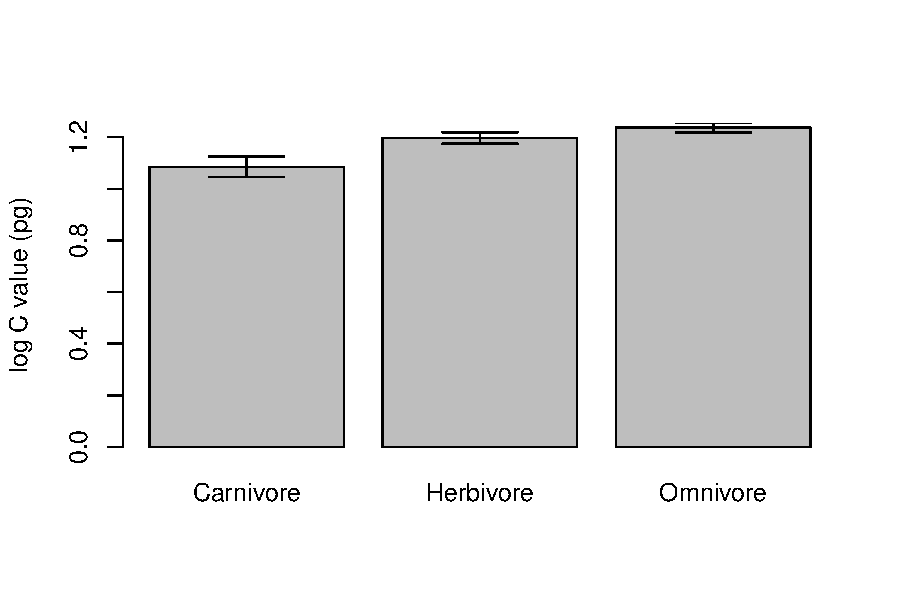
\includegraphics[width=0.7\textwidth]{TLbarplot.pdf}
\end{center} 

Now we need to draw all these pieces together into a script and get 
used to using them.
\begin{compactitem}[$\quad\star$]
	\item Copy all the lines of code from this section into your script.
	\item Run it and check you get the graph above.
	\item Use the second two chunks as a model to plot a similar graph 
	for {\tt GroundDwelling}. You should get something like the plot 
	below.
\end{compactitem}

\begin{center}
	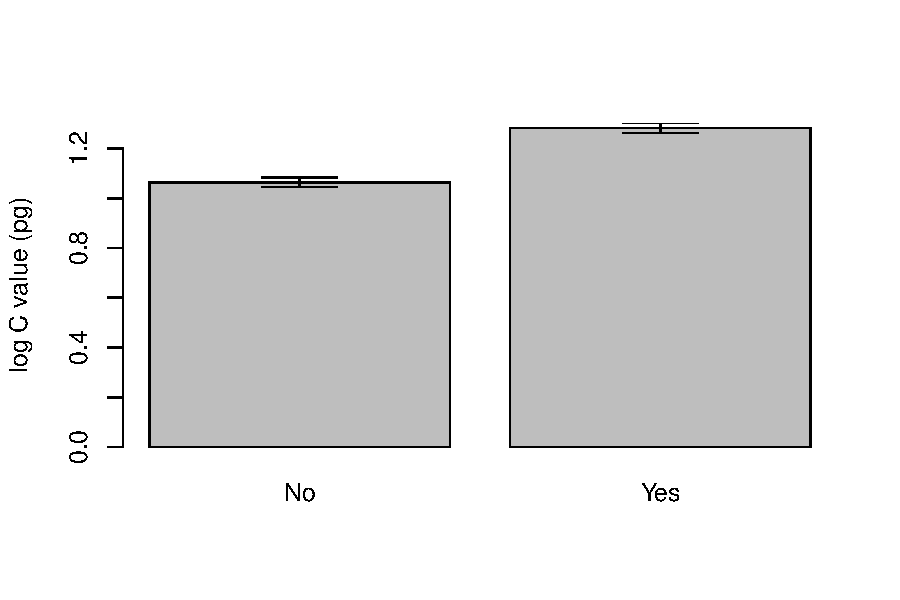
\includegraphics[width=0.6\textwidth]{GDbarplot.pdf}	
\end{center}
 
\section{An alternative to barplots}

That is a lot of work to go through for a plot. Doing it the hard way 
uses some useful tricks, but one strength of R is that there is a huge 
list of add-on packages that you can use to get new functions that 
other people have written.

We will use the {\tt gplots} package to create  plots of group means 
and confidence intervals. Rather than plotting the means $\pm$ 1 
standard error, the option {\tt p=0.95} uses the standard error and the 
number of data points to get 95\% confidence intervals. The default 
{\tt connect=TRUE} option adds a line connecting the means, which isn't 
useful here. 

\begin{compactitem}[$\quad\star$]
	\item Replicate the code below into your script and run it to get the 
	plots below.
\end{compactitem}

\begin{lstlisting}
#Load the gplots package
> library(gplots)

# Get plots of group means and standard errors
> par(mfrow=c(1,2))
> plotmeans(logCvalue ~ TrophicLevel, data=mammals, p=0.95, connect=FALSE)
> plotmeans(logCvalue ~ GroundDwelling, data=mammals, p=0.95, connect=FALSE)
\end{lstlisting}


\begin{center}
	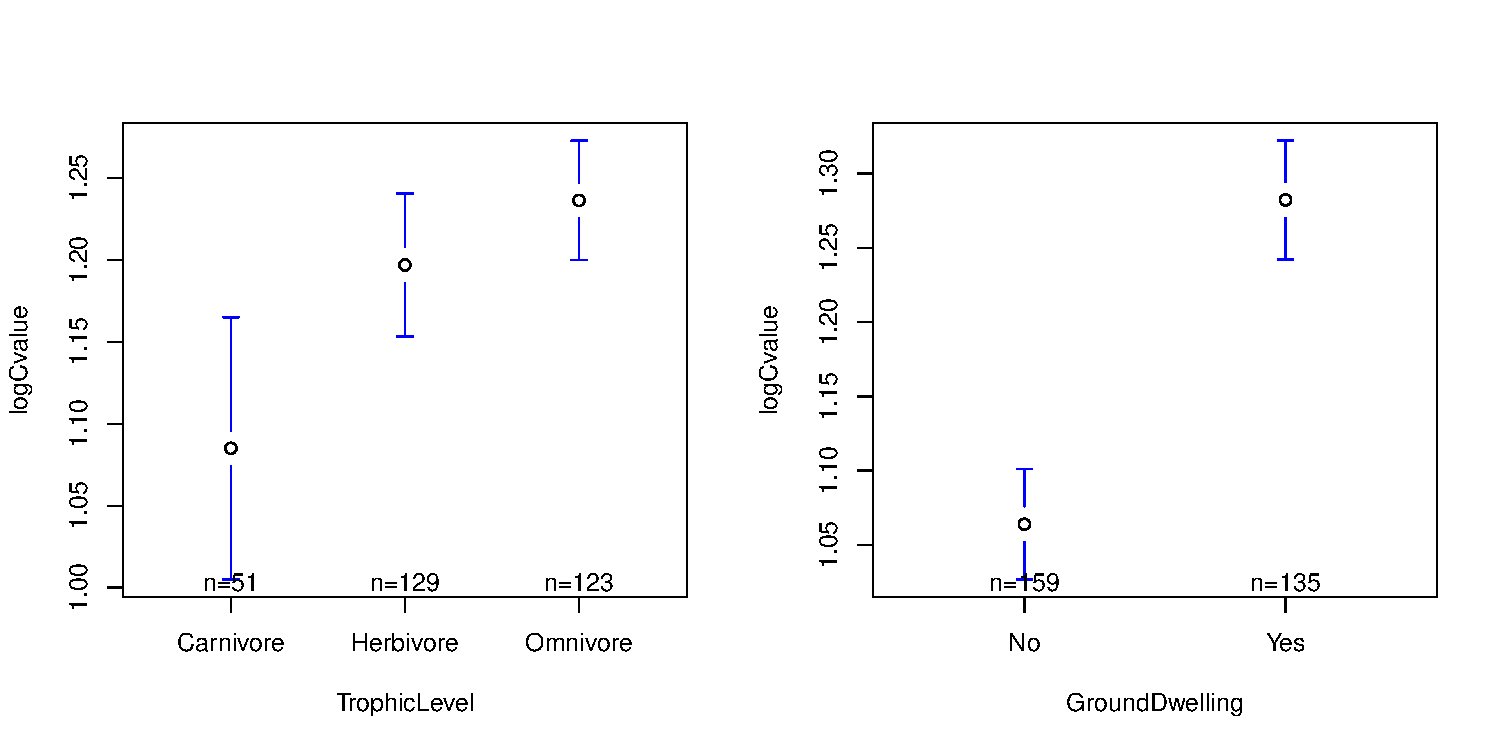
\includegraphics[width = \textwidth]{test.pdf}	
\end{center}

\section{Analysis of variance}

Hopefully, those plots should convince you that there are differences 
in genome size between different trophic groups and between ground 
dwelling and other mammals. We'll now use a linear model to test 
whether those differences are significant.

\begin{compactitem}[$\quad\star$]
	\item Using your code from Chapter~\ref{ch:regress} as a guide, 
	create a linear model called {\tt trophicLM} which models log C value 
	as a function of trophic group.
	\item Use {\tt anova} and  {\tt summary} to look at the analysis of 
	variance table and then the coefficients of the model. 
\end{compactitem}

The ANOVA table for the model should look like the one below: trophic 
level explains highly significant variation in genome size ($F= 7.22, 
\textrm{df}=2 \textrm{ and } 300, p =0.0009$). {\it Note the style of 
reporting the result} - the statistic ($F$), degrees of freedom and $p$ 
value are all provided in support. It is common to contract this style 
to this: $F_{2,300}=7.22, p=0.0009$. 
\begin{lstlisting}
> anova(trophicLM)
 
 Analysis of Variance Table
 
 Response: logCvalue
               Df Sum Sq Mean Sq F value  Pr(>F)    
 TrophicLevel   2   0.83   0.413    7.22 0.00087 ***
 Residuals    300  17.18   0.057                    
 ---
 Signif. codes:  0 '***' 0.001 '**' 0.01 '*' 0.05 '.' 0.1 ' ' 1 

\end{lstlisting}

However, look at the sum of squares column. Of a total of $17.18+0.83 = 
18.01$ units of sums of squares, only 0.83 are explained by trophic 
level: $0.83/18.01 \approx 0.046$ or 4.6\%. This ratio is called 
$r^2$, a measure of explanatory power, and shows that, although the 
model is very significant, it isn't very explanatory. We  care about 
explanatory power or effect size, {\it not} $p$ values.
  
The coefficients table for the model looks like this:

\begin{lstlisting}
> summary(trophicLM)
 
 Call:
 lm(formula = logCvalue ~ TrophicLevel, data = mammals)
 
 Residuals:
     Min      1Q  Median      3Q     Max 
 -0.5038 -0.1635 -0.0038  0.1511  0.9313 
 
 Coefficients:
                       Estimate Std. Error t value Pr(>|t|)    
 (Intercept)             1.0851     0.0335   32.38  < 2e-16 ***
 TrophicLevelHerbivore   0.1119     0.0396    2.83  0.00503 ** 
 TrophicLevelOmnivore    0.1513     0.0399    3.80  0.00018 ***
 ---
 Signif. codes:  0 '***' 0.001 '**' 0.01 '*' 0.05 '.' 0.1 ' ' 1 
 
 Residual standard error: 0.239 on 300 degrees of freedom
   (76 observations deleted due to missingness)
 Multiple R-squared: 0.0459,	Adjusted R-squared: 0.0396 
 F-statistic: 7.22 on 2 and 300 DF,  p-value: 0.000866 
 
\end{lstlisting} 

It shows the following:

\begin{compactitem}

	\item The reference level (or intercept) is for carnivores. Their 
	mean genome size is significantly different from zero - this is not 
	an exciting finding!

	\item The mean genome size for both herbivores and omnivores are both 
	significantly different from carnivores. Both larger in fact: 
	herbivore mean genome size = $1.085 + 0.112 = 1.197$ and omnivore 
	mean genome size = $1.085 + 0.151 = 1.236$. These are the same group 
	means we found above.

	\item The $r^2$ is shown and is the 4.6\% we calculated above. The 
	{\it adjusted} $r^2$ reduces the raw $r^2$ to account for the number 
	of variables included in the model. That 4.6\% would be even less 
	impressive if we needed 6 explanatory variables to get it\ldots

	\item The $F$ statistic, as in the ANOVA table above.

\end{compactitem}

\begin{compactitem}[$\quad\star$]
	\item Repeat the analysis of variance above to look at the effects of 
	ground dwelling on genome size.
\end{compactitem}

\section{Model criticism}

The next question must be  ---  and actually, we should do this before 
we go anywhere near the model summaries --- is the model appropriate to 
the data.

\begin{compactitem}[$\quad\star$]
	\item Using Chapter \ref{ch:regress} to guide you, get the four model 
	diagnostic plots for the trophic level model on a single figure.
\end{compactitem}

The four plots are:
\begin{center}
	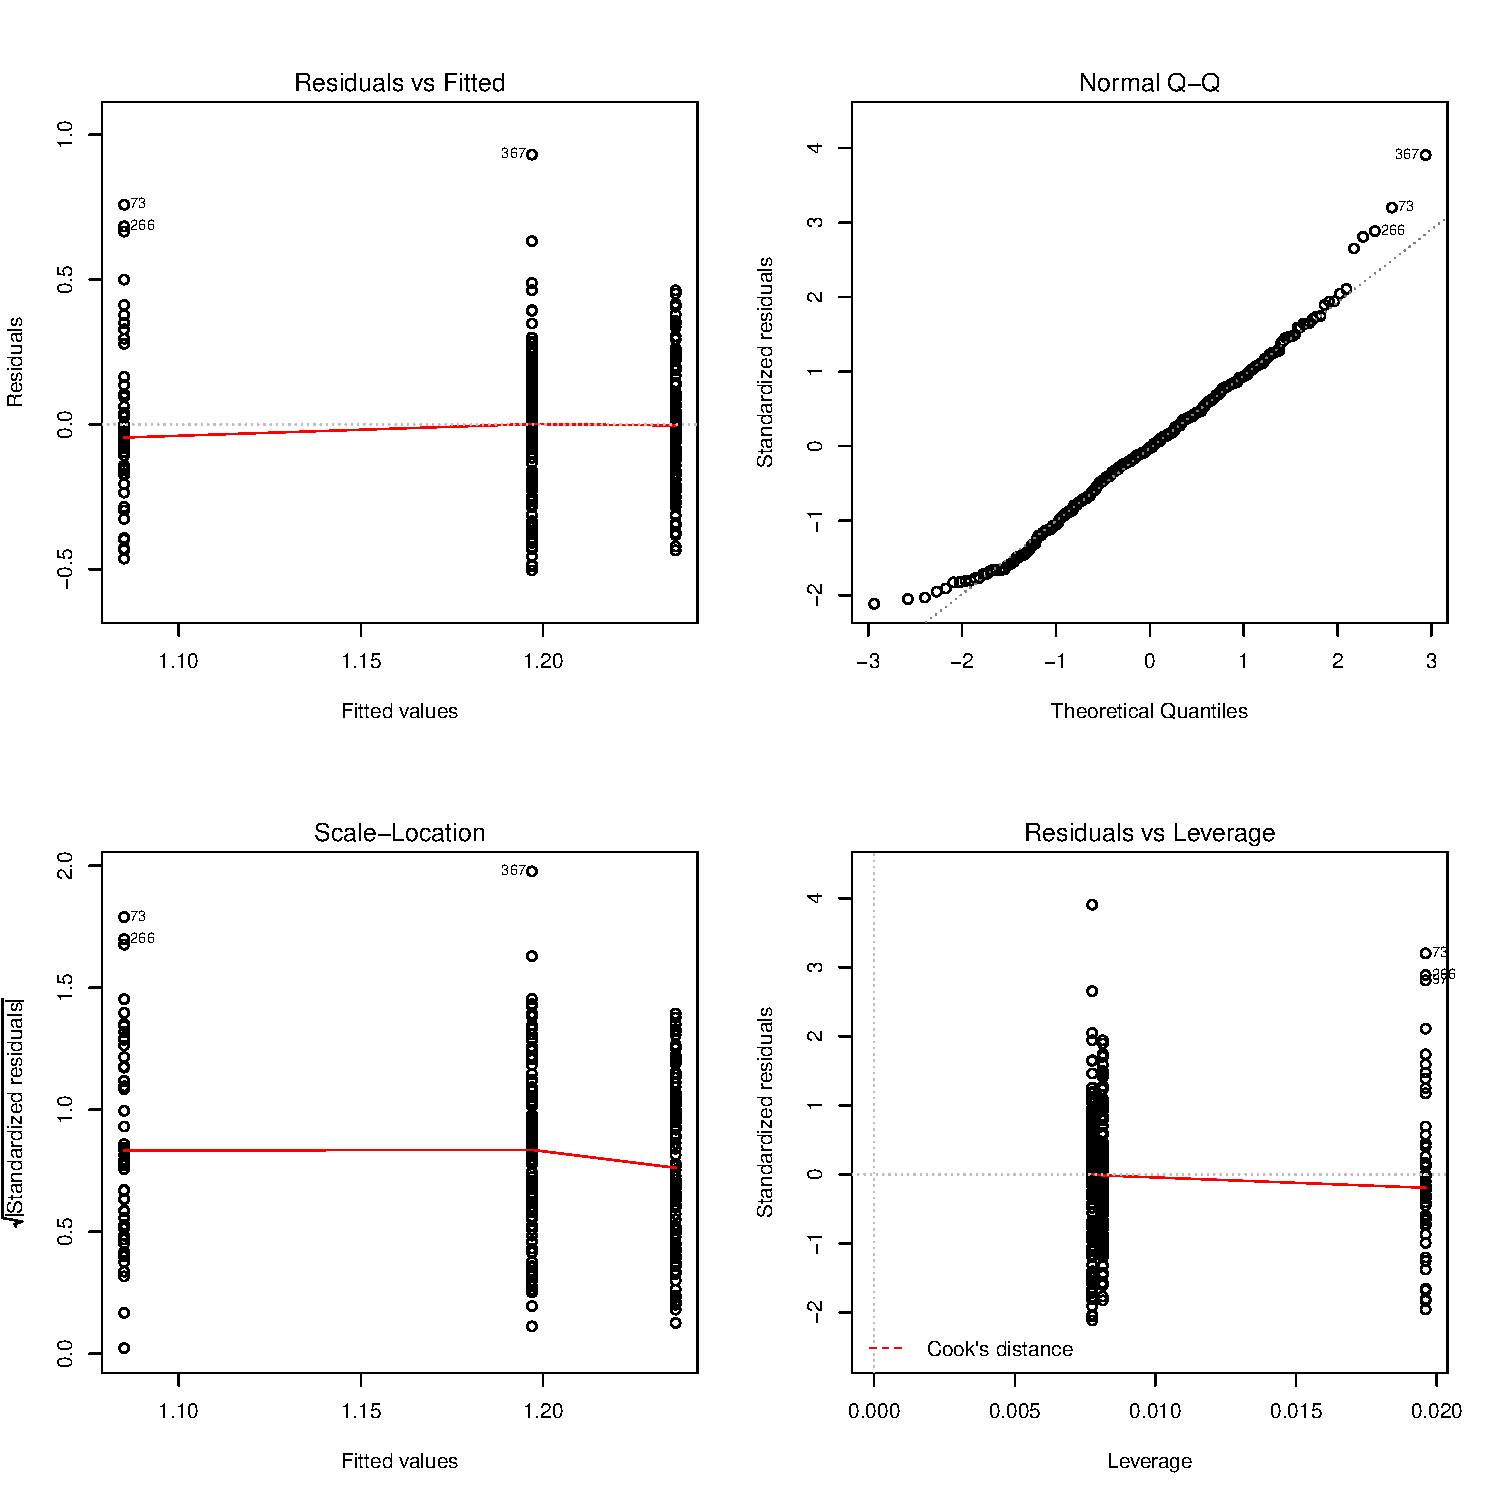
\includegraphics[width=0.8\textwidth]{modelDiag.pdf}	
\end{center}

Note that in regression, the predicted (or fitted) values from the 
model take a range along the relationship $y=a + bx$ (as we saw in the 
Figures \ref{fig:DiagModDragon} \& \ref{fig:DiagModDamsel}). For ANOVA, 
there are only a few predicted values --- one for each group mean. This 
means that the plots above look different but we are looking for the 
same things: is there constant variance at each fitted value and are 
the residuals normally distributed? The answer for this model looks to 
be yes.

\begin{compactitem}[$\quad\star$]
	\item Check the ground dwelling model in the same way.
\end{compactitem}
 
\section{Testing pairwise differences between levels}

The one thing that the trophic level model does not tell us is whether 
there is a difference in genome size between omnivores and herbivores 
--- both are compared to carnivores, but not to each other. This is 
because of the multiple pairwise testing problem mentioned in Chapter 
\ref{ch:t_F_tests} --- if you do 
lots of tests then you may find small $p$ values by chance and say 
something important is going on when it is just random chance. This is 
called a false positive or Type I error.
 
With a 95\% confidence interval, there is a 5\% chance of a false 
positive {\it per test} but there are ways of getting a 5\% chance 
across a set (or family) of tests. For  linear models, we can use 
Tukey's Honest Significant Difference test. We have to convert the {\tt 
lm} object into an {\tt aov} object first.

\begin{lstlisting}

> TukeyTroph <- TukeyHSD(aov(trophicLM))
> print(TukeyTroph)
	
   Tukey multiple comparisons of means
     95% family-wise confidence level
 
 Fit: aov(formula = trophicLM)
 
 $TrophicLevel
                        diff      lwr    upr  p adj
 Herbivore-Carnivore 0.11186  0.01863 0.2051 0.0139
 Omnivore-Carnivore  0.15128  0.05741 0.2452 0.0005
 Omnivore-Herbivore  0.03942 -0.03161 0.1104 0.3923
 
\end{lstlisting}

The table shows the following:
\begin{compactitem}

	\item The differences between the three possible pairs and then the 
	lower and upper bounds of the 95\% confidence interval for the 
	difference and a $p$ value. 

	\item In each case, we want to know if the difference could be zero: 
	does the 95\% confidence interval for each pair include zero.

	\item For the first two pairs,  carnivores versus omnivores and 
	herbivores, the confidence intervals do not include zero, so they are 
	significantly different. For the comparison between herbivores and 
	omnivores, the interval does include zero (difference = 0.039, 95\% 
	CI's limits are -0.032 \& 0.110), so these groups are not 
	significantly different.

	\item The $p$ values for the top two pairs are both larger (less 
	significant) than in the summary table. The test has made it harder 
	to find significant results.

\end{compactitem}

You can visualise these confidence intervals by plotting the Tukey 
test. You have to tweak the graphics parameters to get a clean plot 
though.

\begin{lstlisting}
> par(las=1, mar=c(4,10,3,1))
# las= 1 turns labels horizontal
# mar makes the left margin wider (bottom, left, top, right)
> plot(TukeyTroph)
\end{lstlisting} 

The result should be:

{\centering 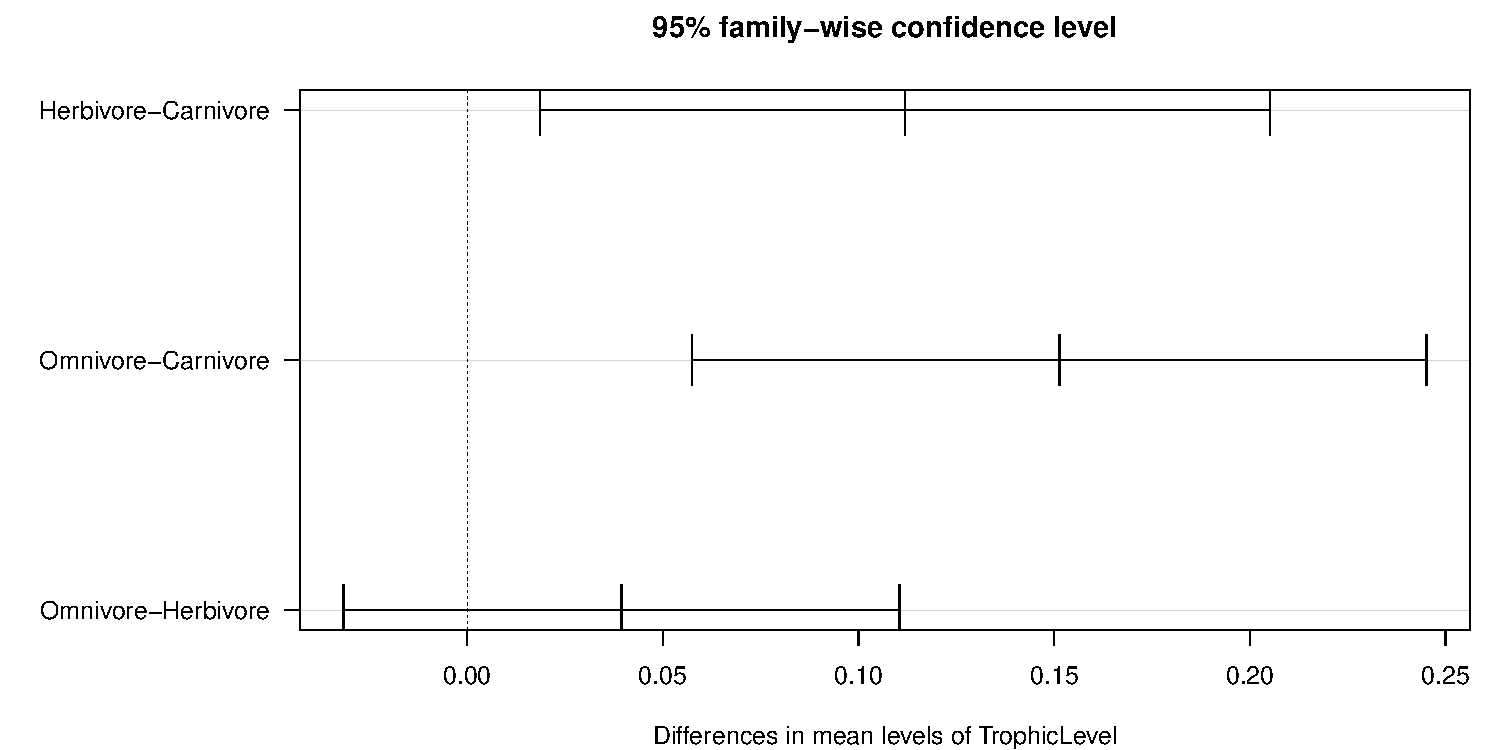
\includegraphics[width=0.8\textwidth]{TukeyPLot.pdf} }

\begin{compactitem}[$\quad\star$]
	\item Run the Tukey test in your script for both the trophic level 
	and ground dwelling models.
\end{compactitem}

\section{Are the factors independent?}

We've looked at two models, using trophic level and ground dwelling. It 
is worth asking whether these are independent factors. What if, for 
example, our herbivores are all big, ground dwellers? This is important 
to know because otherwise, a two-way ANOVA would not be appropriate. We 
will look at interactions in Chapter \ref{ch:MulExplInter}.

OK, so we want to know whether the two factors are independent. This is 
a job for the $\chi^2$ test!

\subsection{The Chi-square test and count data}

The Chi-square test, also known as $\chi^{2}$ test or chi-square test, 
is designed for scenarios where you want to statistically test how 
likely it is that an observed distribution of values is due to chance. 
It is also called a ``goodness of fit'' statistic, because it measures 
how well the observed distribution of data fits with the distribution 
that is expected if the variables of which measurements are made are 
independent. In our mammals example below, the two variables are 
trophic level and ground dwelling.

Note that a $\chi^{2}$ test is designed to analyze categorical data. 
That is the data have been counted (count data) and divided into 
categories. It is not meant for continuous data (such as body weight, 
genome size, or height). For example, if you want to test whether 
attending class influences how students perform on an exam, using test 
scores (from 0-100) as data would not be appropriate for a Chi-square 
test. However, arranging students into the categories ``Pass'' and 
``Fail'' and counting up how many fall in each categories would be 
appropriate. Additionally, the data in a Chi-square table (see below) 
should not be in the form of percentages -- only count data are 
allowed! 

\subsubsection{The Chi-square test with the mammals data}

We can easily build a table for a Chi-square test on the mammals 
data as follows:
  
\begin{lstlisting}
> factorTable <- table(mammals$GroundDwelling, mammals$TrophicLevel)
> print(factorTable) 

       Carnivore Herbivore Omnivore
   No         26        45       64
   Yes        22        62       40
\end{lstlisting}

Now let's run the test:

\begin{lstlisting}
> chisq.test(factorTable)
  
 	Pearson's Chi-squared test
 
 data:  factorTable 
 X-squared = 8.12, df = 2, p-value = 0.01725
\end{lstlisting}

The ``{\tt X-squared}'' value is the $\chi^{2}$ {\it test statistic}, akin to the 
t-value of the t-test or W value in the Wilcox test. 

The $\chi^{2}$ statistic is calculated as the sum of the quantity 
$$ \frac{(\mathrm{Observed} - \mathrm{Expected})^2}{\mathrm{Expected}} $$
across all the cells/categories in the table (so the sum would be over 
6 categories in our current mammals example).
   
``Observed'' is the observed proportion of data that fall in a 
certain category. For example, there are 26 species observed in the 
{\tt Carnivore}, {\tt No} category, and 22 in the {\tt Carnivore}, {\tt 
Yes} category. 

``Expected'' is what count would be expected if the values in each 
category we truly independent. Each cell has its own expected value, 
which is simply calculated as the count one would expect in each 
category if the value were generated in proportion to the total number 
seen in that category. So in our example, the expected value for the 
{\tt Carnivore}, {\tt No} category would be
$$26+22 \mathrm{~(Total~number~of~carnivore~species)} 
\times \frac{26+45+64 \mathrm{~(Total~number~in~the~''No''~category)}}{ 
26+22+45+62+64+40 \mathrm{~(Total~number~of~species)}}$$  
$$= 48 \times \frac{135}{259} = 25.02$$

The sum of all six (one for each cell in the table above) such 
calculations would be the $\chi^{2}$ value that R gave you through the 
{\tt chisq.test()} above --- try it!

Now back to the R output from the {\tt chisq.test()} above. Why df = 2? 
This is calculated as $DF = (r - 1) * (c - 1)$ where $r$ and $c$ are 
the number of rows and columns in the $\chi^{2}$ table, respectively. 
The same principle you learned before applies here; you lose one degree 
of freedom for each new level of information you need to estimate: 
there is uncertainity about the information (number of categories) in 
both rows and columns, so you need to lose one degree of freedom for 
each. 

Finally, note that the p-value is significant --- we can conclude that the 
factors aren't independent. From the table, carnivores can be either 
ground dwelling or not, but herbivores tend to be ground dwelling and 
omnivores tend not to be. Ah well... it's OK. We will look at a better 
way to analyze these data using ``interactions'' in Chapter 
\ref{ch:MulExplInter}.

\begin{compactitem}[$\quad\star$]
	\item Include and run the $\chi^2$ test in your script.
\end{compactitem}

\section{Saving data}

The last thing to do is to save a copy of the mammal data, including 
our new column of log data, for use in later chapters. 

\begin{compactitem}[$\quad\star$]
	\item Use this code in your script to create the saved data in you 
	{\tt Data} directory :
\end{compactitem}

\begin{lstlisting}
save(mammals, file='../Data/mammals.Rdata')
\end{lstlisting}	
